\documentclass[dvipsnames,
%xcolor={svgnames},
hyperref={citecolor=black}
]{beamer}
\beamertemplatenavigationsymbolsempty
\usetheme{Boadilla}
\usefonttheme[onlymath]{serif}

\usepackage{cleveref}

\usepackage{amsmath}
\usepackage{bm}
\usepackage{bbm}
\usepackage{mathrsfs}
\usepackage{mathtools}
\usepackage[cal=boondoxo]{mathalpha}

% Change horizontal spacing
\setlength{\tabcolsep}{3pt}

\usepackage[none]{hyphenat} % no hyphenation

\usepackage{array}

\usepackage{cancel}

\usepackage[style=authoryear,maxcitenames=2,backend=biber,citetracker=true]{biblatex}
\addbibresource{references.bib}

\usepackage{verbatim}

\usepackage{bigints}

\DeclareCiteCommand{\citeauthor}
{\boolfalse{citetracker}%
	\boolfalse{pagetracker}%
	\usebibmacro{prenote}}
{\ifciteindex
	{\indexnames{labelname}}
	{}%
	\printtext[bibhyperref]{\printnames{labelname}}}
{\multicitedelim}
{\usebibmacro{postnote}}

\DeclareCiteCommand{\citeyear}
{\usebibmacro{prenote}}
{\bibhyperref{\printfield{year}}\bibhyperref{\printfield{extrayear}}}
{\multicitedelim}
{\usebibmacro{postnote}}

\newcommand{\credit}[2]{{\par\hfill \tiny #1 credit:~\itshape\citeauthor{#2} (\citeyear{#2})}}
\renewcommand{\cite}[1]{(\citeauthor{#1}, \citeyear{#1})}
\newcommand{\citefoot}[1]{\citeauthor{#1} (\citeyear{#1})}
\newcommand{\matr}[1]{#1}

\newcommand{\red}[1]{{\color{red} #1}}

\title[ProLLaMA]
{\href{https://doi.org/10.48550/arXiv.2402.16445}{ProLLaMA: A Protein Large Language Model for Multi-Task Protein Language Processing}}
%\subtitle{}
\author[Liuzhenghao Lv et al.]{Lv, Liuzhenghao, Zongying Lin, Hao Li, Yuyang Liu, Jiaxi Cui, Calvin Yu-Chian Chen, Li Yuan, and Yonghong Tian
\\\vspace{2em}Presenter: Gianmarco Midena}
%\institute{Aalto University}
\date[3 July 2024]{Submitted on 26 February 2024 
\\\vspace{2em}3 July 2024}

\begin{document}
\begin{frame}
\titlepage
\end{frame}

%\begin{frame}{Outline}
%\tableofcontents
%\end{frame}

\begin{frame}{Multi-task LLMs for Natural vs. Protein Language}
	\begin{center}
		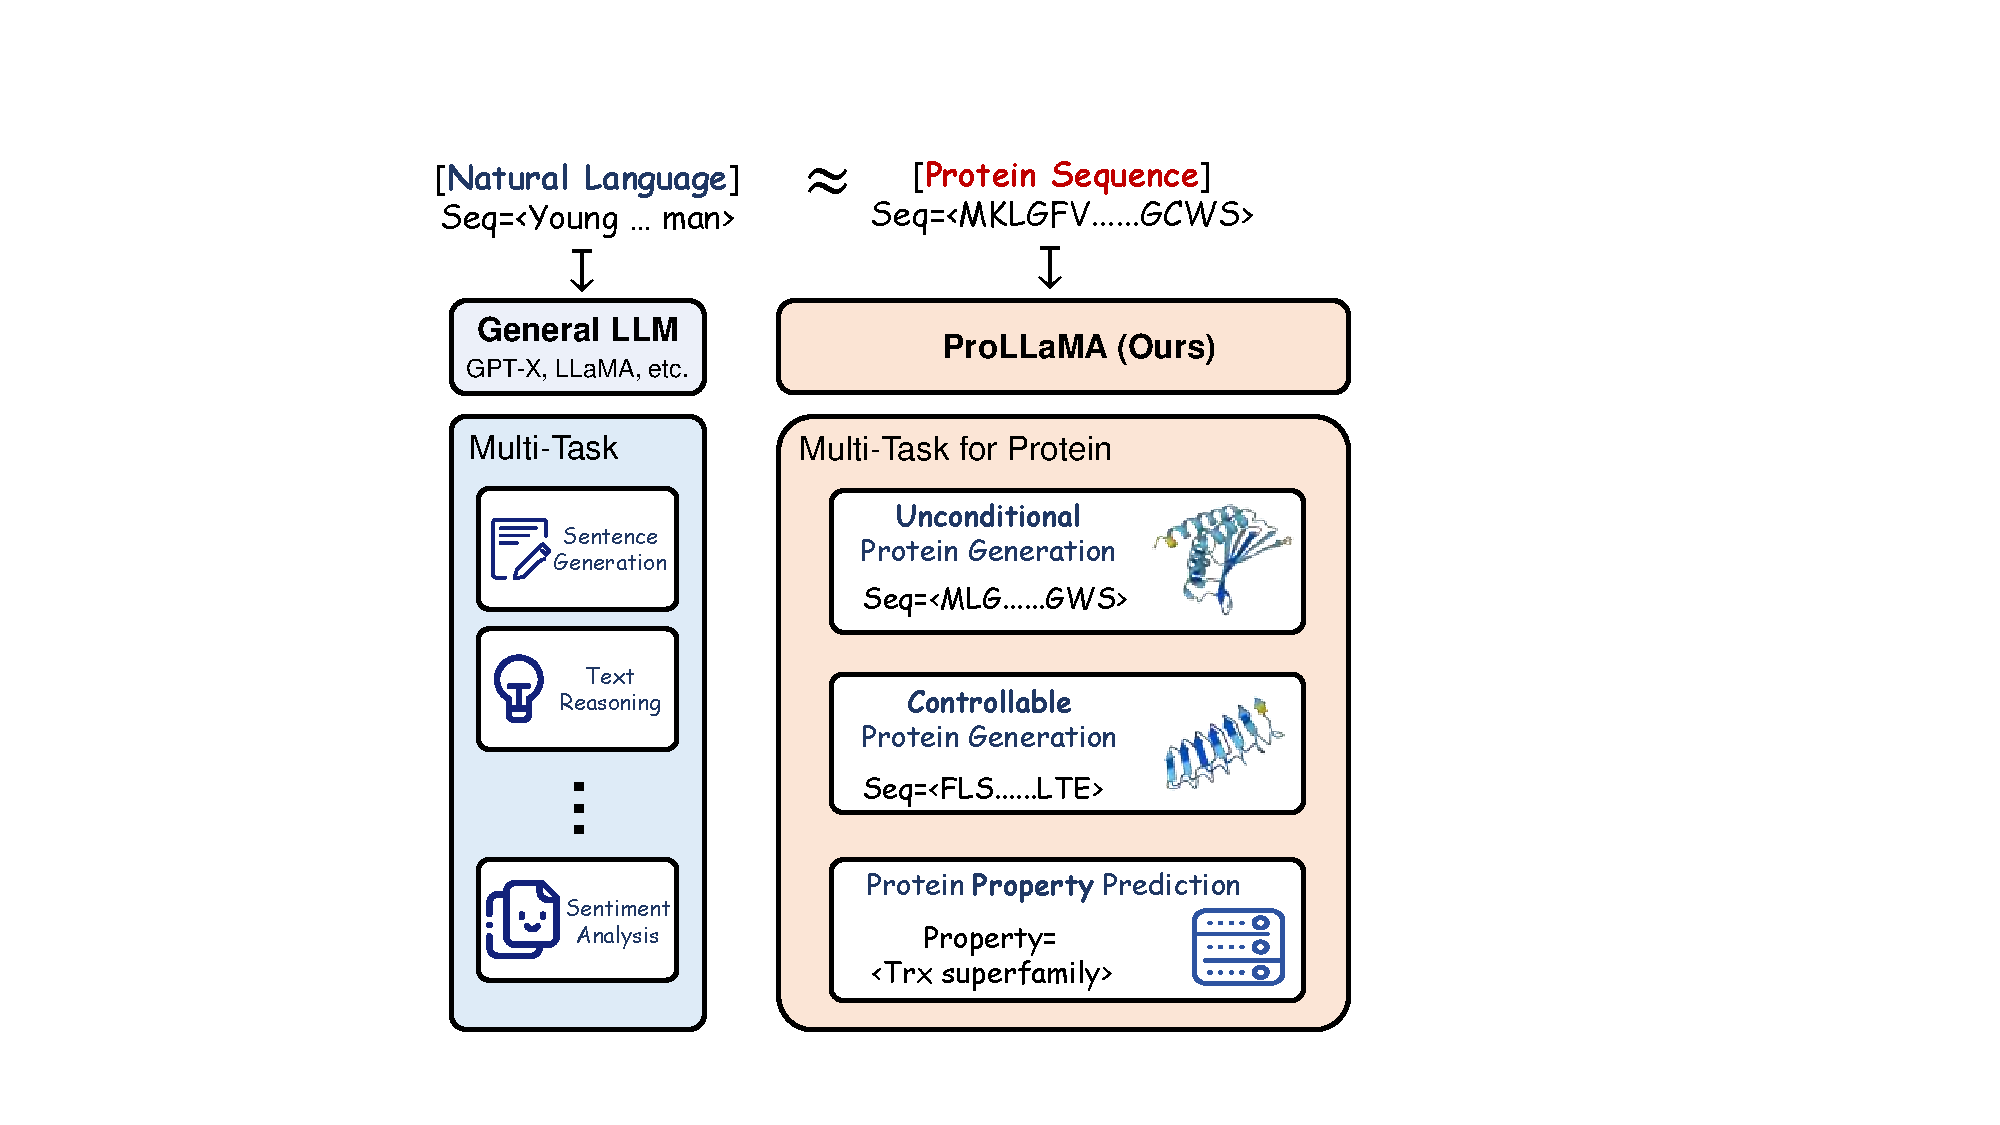
\includegraphics[scale=0.5]{images/multitask_LLMs_NLP_vs_PLP.pdf}
	\end{center}
	\credit{Image}{lv2024prollama}
\end{frame}

\begin{frame}{Model}
	\begin{center}
		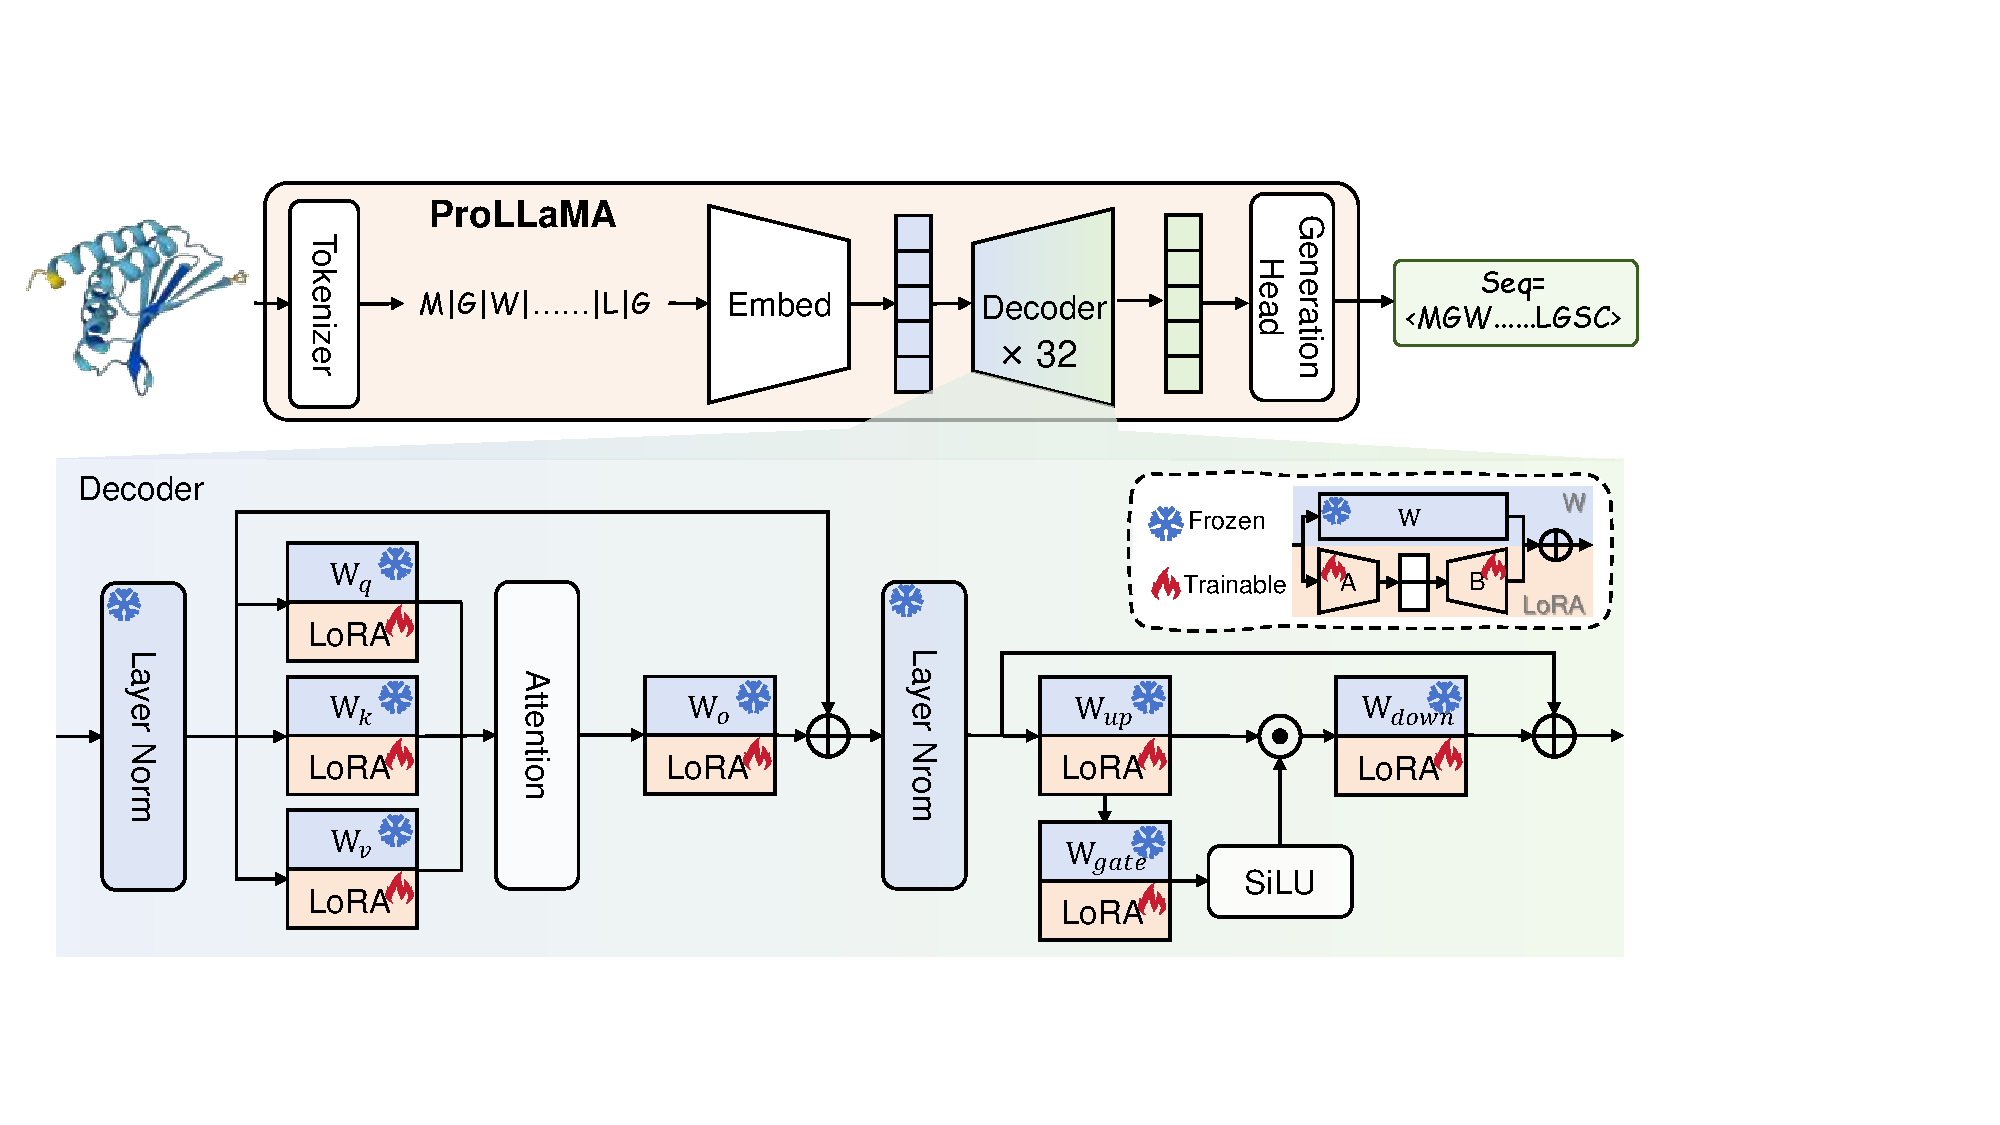
\includegraphics[scale=0.44]{images/model.pdf}
	\end{center}
	\credit{Image}{lv2024prollama}
\end{frame}

\begin{frame}{Learning Stages}
	\begin{center}
		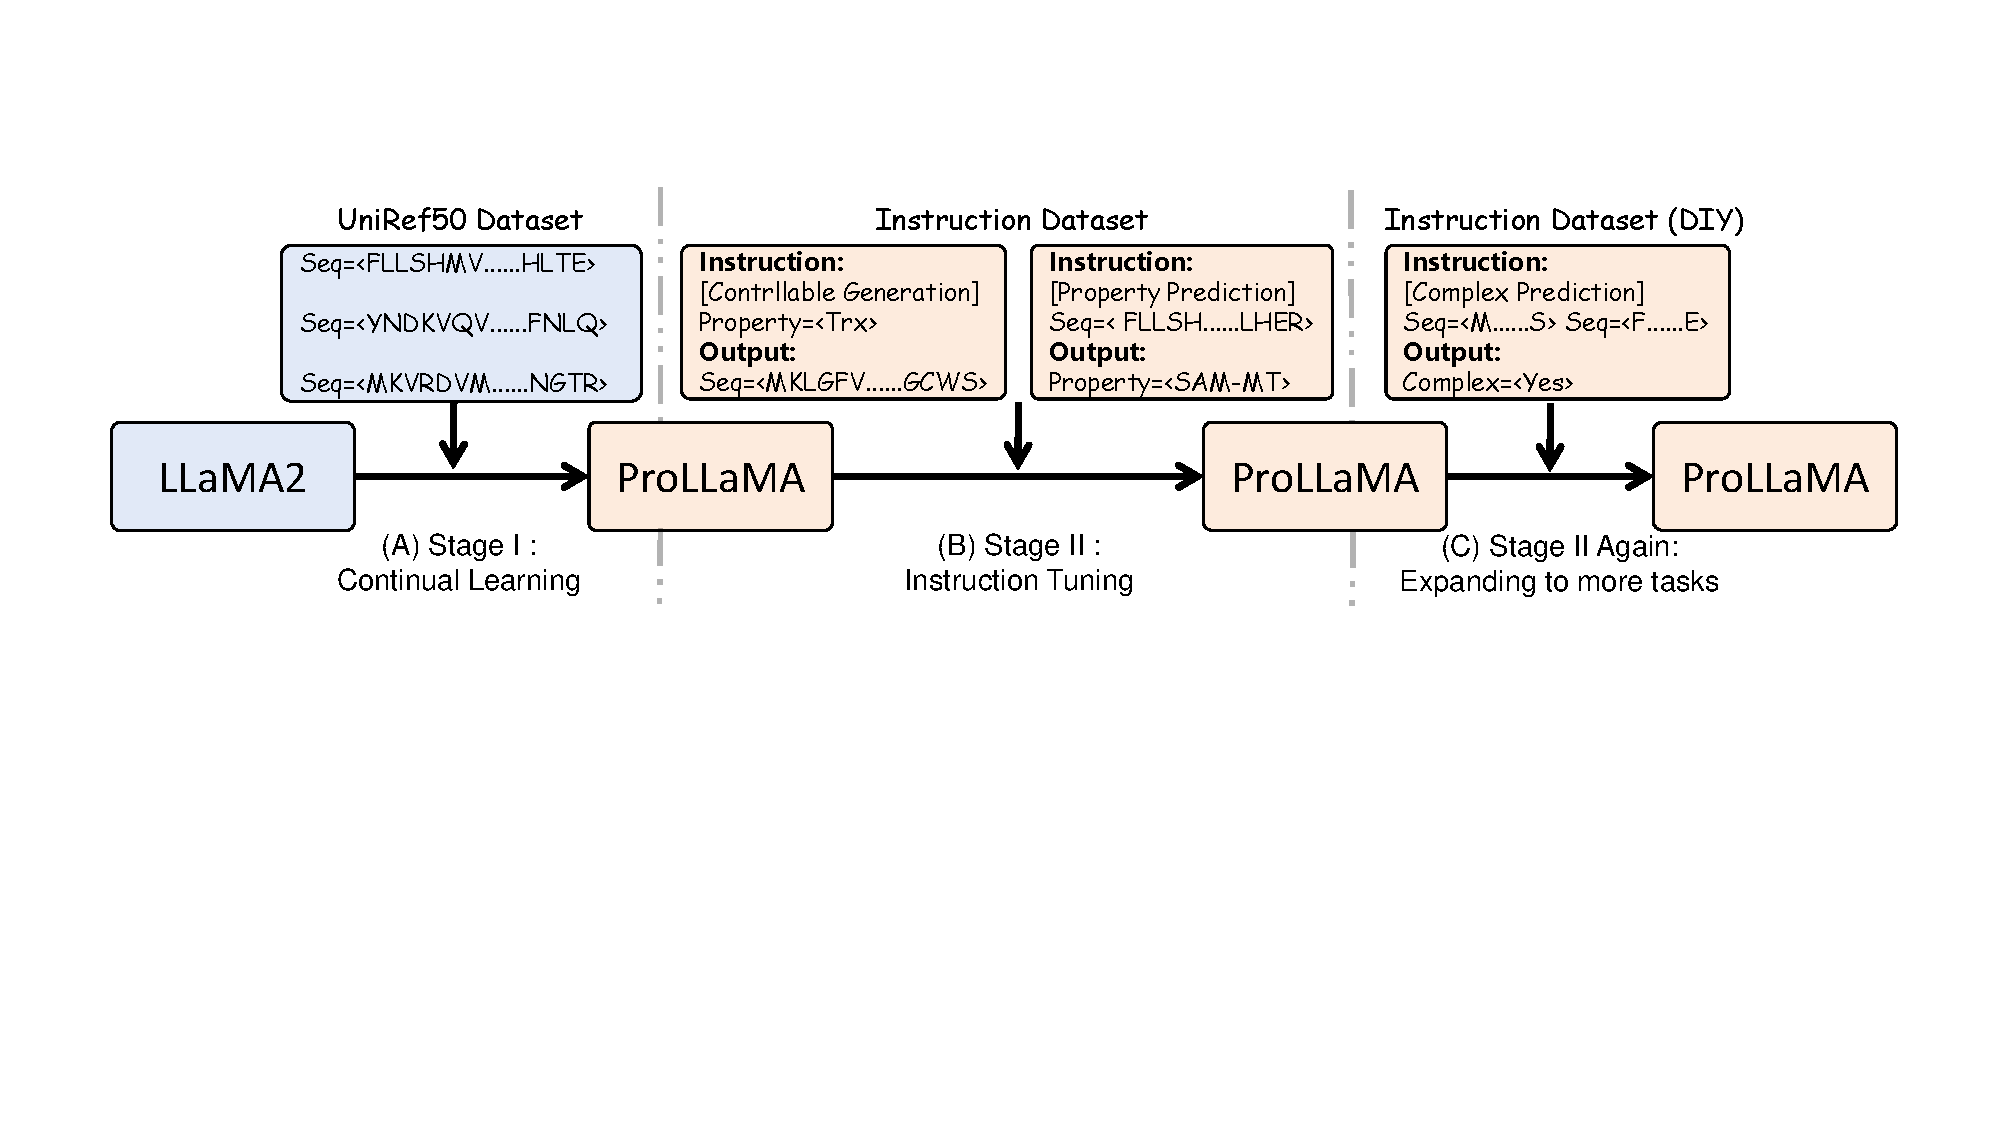
\includegraphics[scale=0.39]{images/training.pdf}
	\end{center}
	\credit{Image}{lv2024prollama}
\end{frame}

\begin{frame}{Evaluation Metrics}
	\begin{itemize}
		\item structural plausibility of a sequence
		\begin{itemize}
			\item \textbf{pLDDT}: Local Distance Difference Test~\cite{jumper2021highly}
			\begin{itemize}
				\item \red{unreliable with Intrinsically Disordered Regions (IDRs)}
			\end{itemize}
			\item \textbf{SC-Perp}: Self-Consistency Perplexity~\cite{alamdari2023protein}
		\end{itemize}
		\item structural similarity between generated and known sequences
		\begin{itemize}
			\item \textbf{TM-score}: Template Modeling score~\cite{zhang2004scoring}
			\item \textbf{RMSD}:  Root-Mean-Square Deviation
			\begin{itemize}
				\item atomic distance
			\end{itemize}
		\end{itemize}
		\item Homologous Probability (\textbf{H-Prob}): probability that a generated protein is homologous to a known one
		%What does homology mean?
		\item Sequence Identity (\textbf{Seq-Ident}): sequence similarity between generated sequences and known ones
	\end{itemize}
\end{frame}

\begin{frame}{Reference Protein Databases}
	\begin{itemize}
		\item AFDB~\cite{varadi2022alphafold}
		\item PDB~\cite{berman2002protein}
	\end{itemize}
\end{frame}

\begin{frame}{Performance in (Unconditional) Protein Generation}
	\begin{center}
		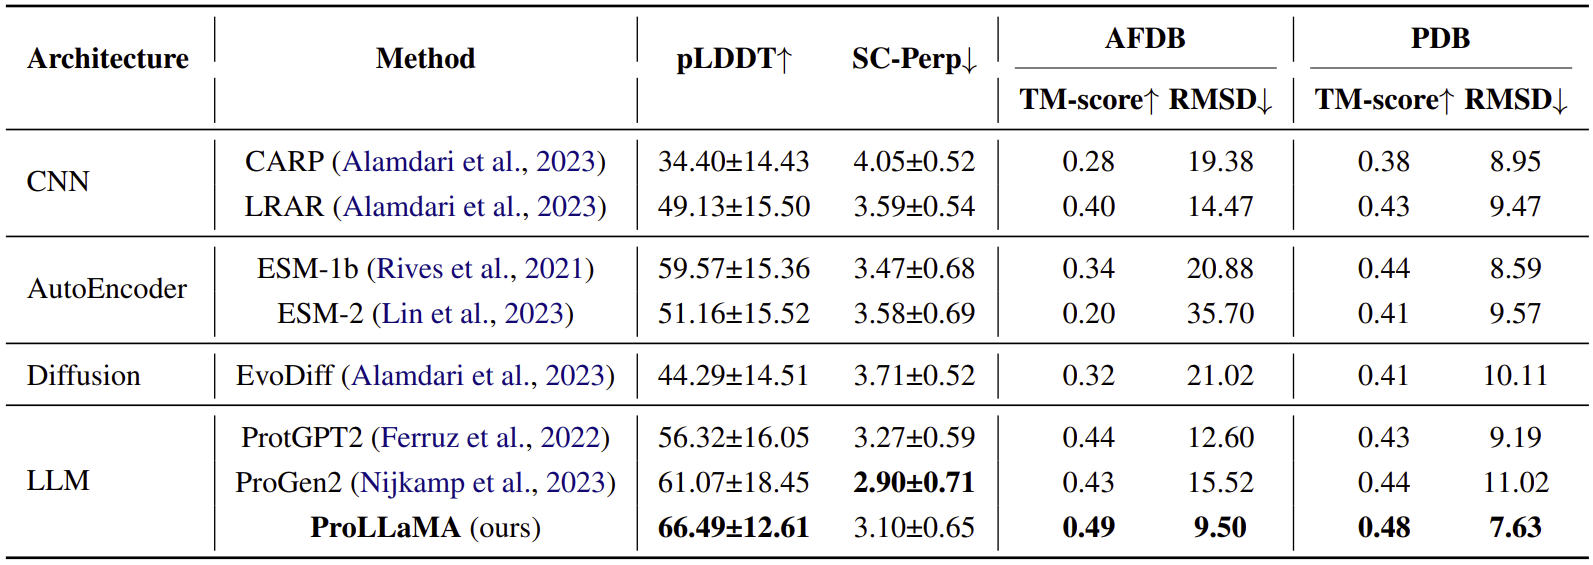
\includegraphics[scale=0.21]{tables/methods_comparison.png}
	\end{center}
	\credit{Table}{lv2024prollama}
\end{frame}

\begin{frame}{Controllable Generation on Four Different Instructions}
	\begin{center}
		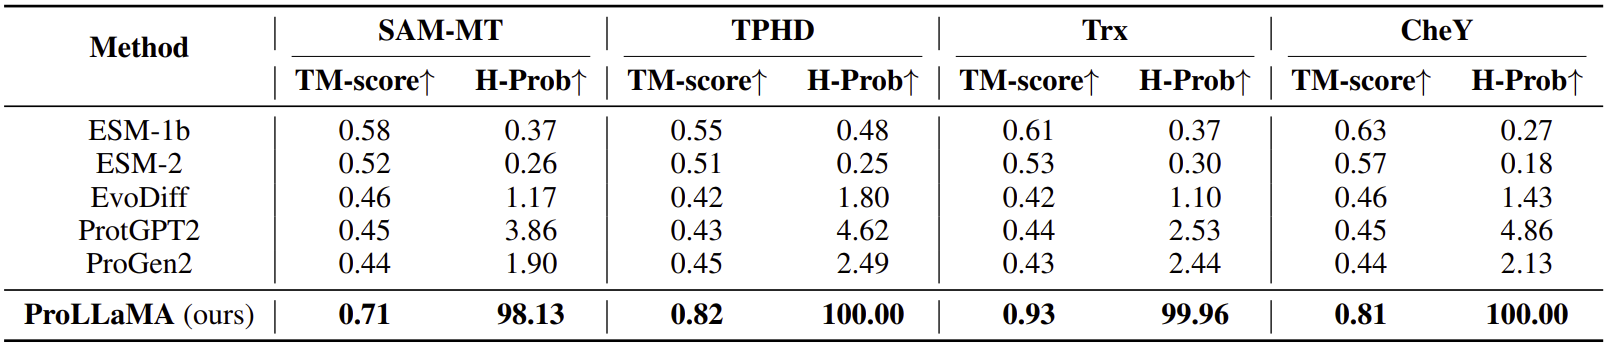
\includegraphics[scale=0.21]{tables/controlled_generation_comparison.png}
	\end{center}
	\vspace{-1em}\credit{Table}{lv2024prollama}
	\begin{itemize}
		\item Given one instruction, \\ProLLaMA generates proteins with the desired functionalities
		\item High metrics mean proteins meet instructions
		\item Other models: uncontrollable generation
		\item Instructions: four superfamily descriptions
		%What do superfamilies are?
		\begin{itemize}
			\item SAM-MT: S-adenosyl-L-methionine-dependent methyltransferase
			\item TPHD: Tetratricopeptide-like helical domain
			\item Trx: Thioredoxin-like 
			\item CheY: CheY-like
		\end{itemize}
	\end{itemize}
\end{frame}

\begin{frame}{Quality of Generated Protein w.r.t. Length}%ProLLaMA vs. ESM2 (Baseline) Model}
	\begin{center}
		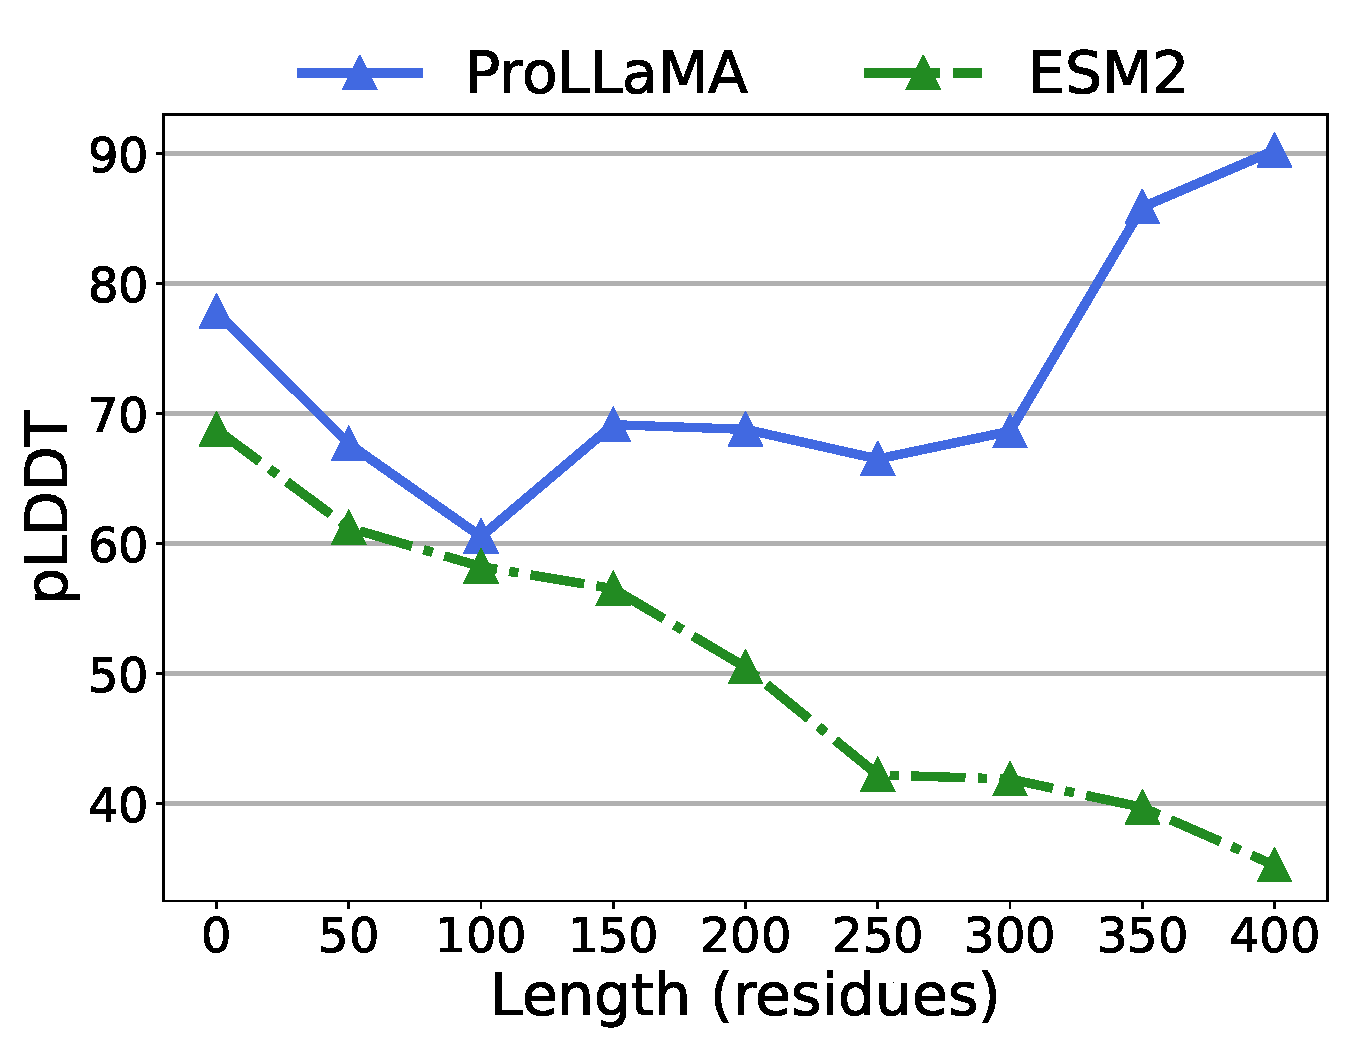
\includegraphics[scale=0.23]{images/combined_length_plddt_zhexiantu.pdf}
		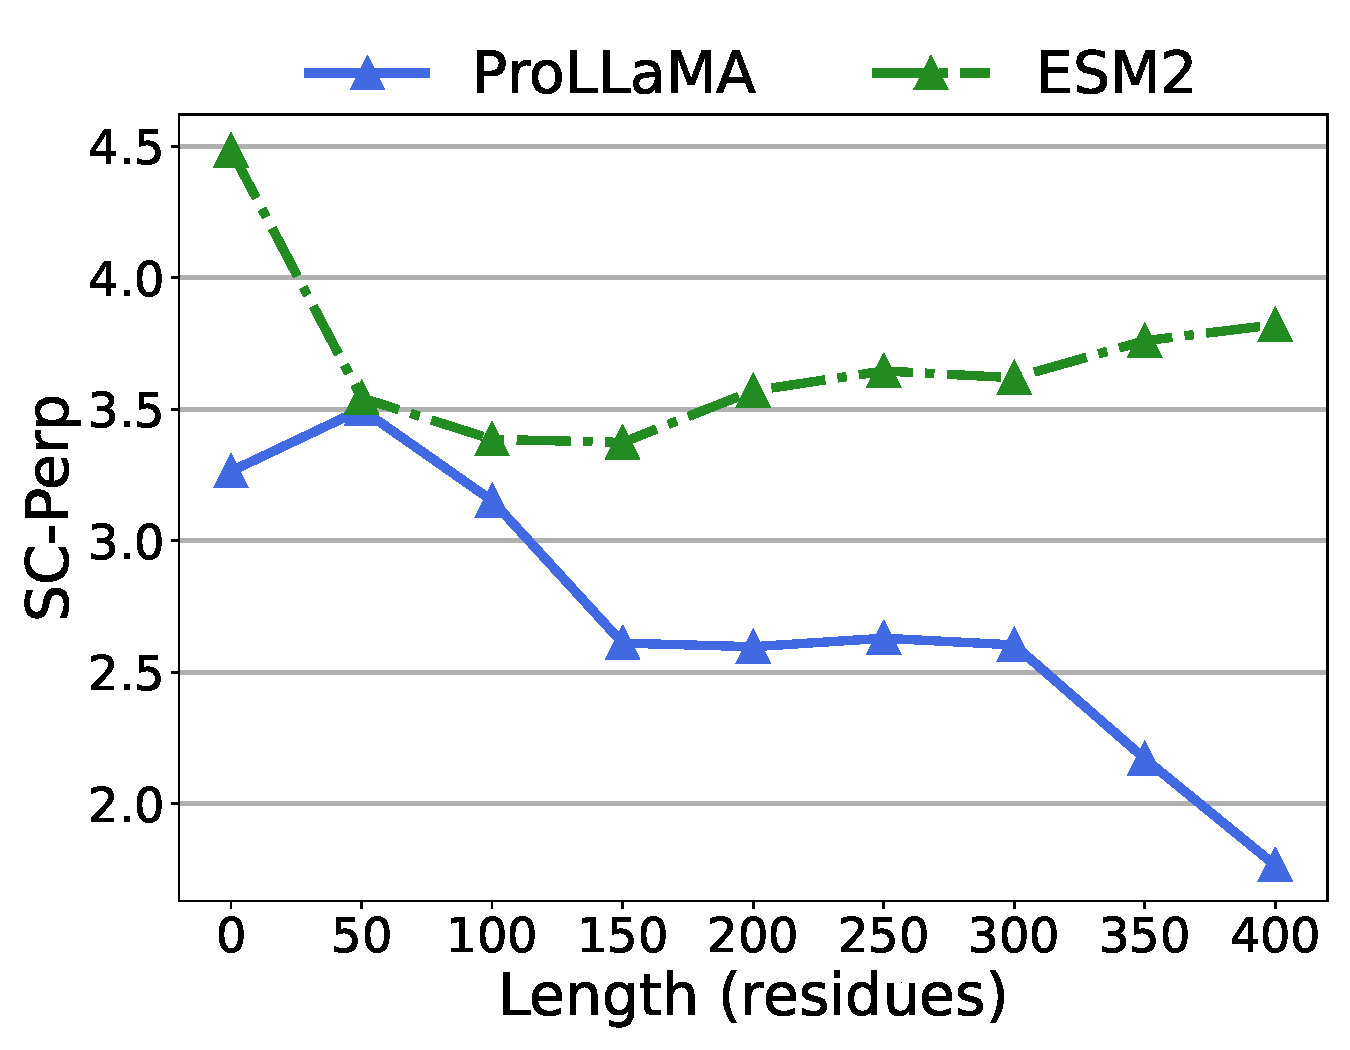
\includegraphics[scale=0.23]{images/combined_length_scperp_zhexiantu.pdf}
		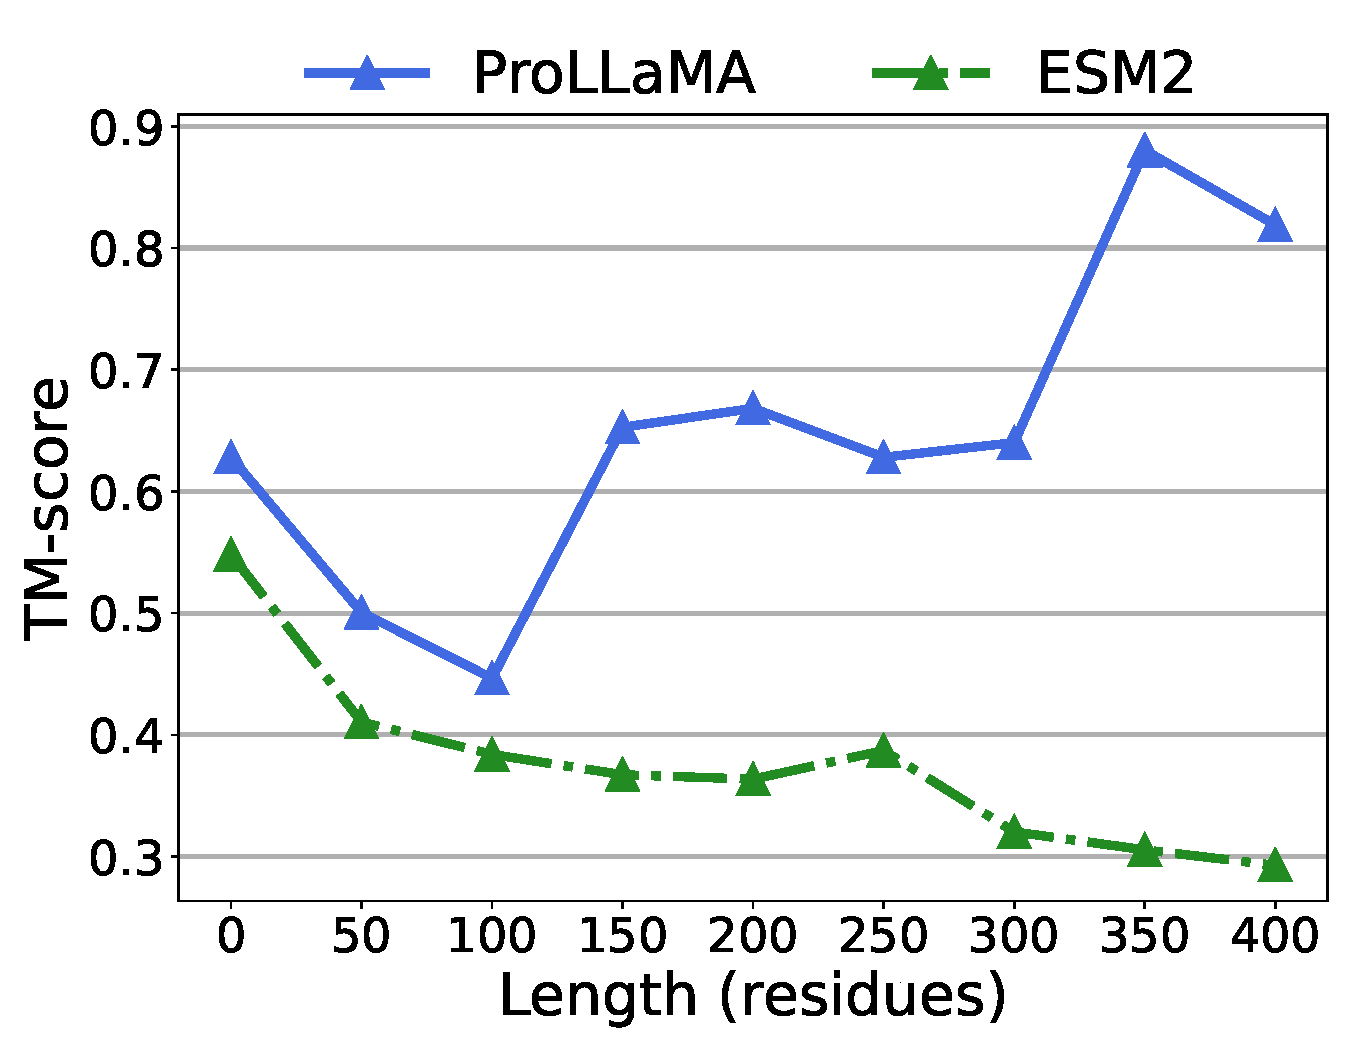
\includegraphics[scale=0.23]{images/combined_length_alntmscore_zhexiantu.pdf}
	\end{center}
	\vspace{-2em}\credit{Image}{lv2024prollama}
\end{frame}

\begin{frame}{Generated vs. Natural Protein}
	\begin{center}
		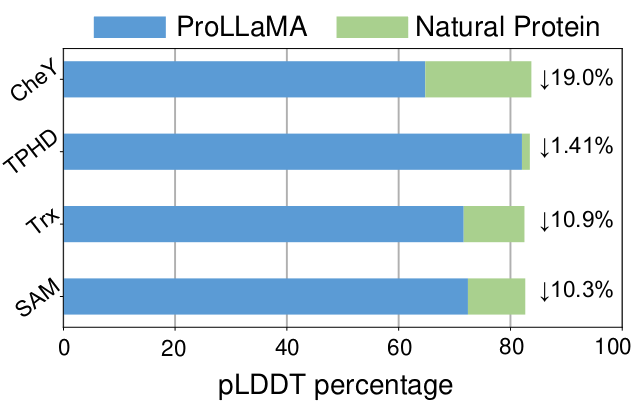
\includegraphics[scale=0.7]{images/d.png}
		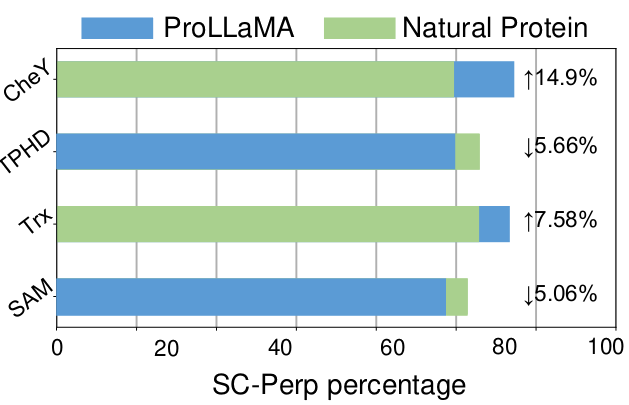
\includegraphics[scale=0.7]{images/e.png}
		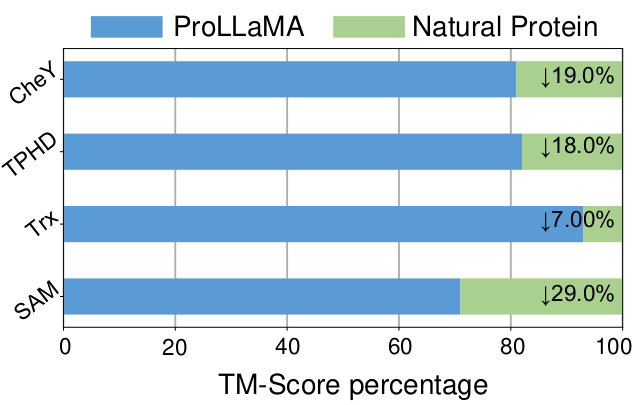
\includegraphics[scale=0.7]{images/f.png}
	\end{center}
	\credit{Image}{lv2024prollama}
\end{frame}

\begin{frame}{Performance in Protein Property Prediction}
	\begin{center}
		\begin{tabular}{cc}\hline
			Property & Accuracy (\%) \\\hline
			OBFD     & 100 \\
			UPF0145  & 100 \\
			NACD     & 100 \\
			U3S      & 100 \\
			CCHC     & 95.24  \\
			Kazal    & 100 \\
			SAM-MT   & 93.67  \\
			TPHD     & 90.84  \\
			Trx      & 94.17  \\
			CheY     & 100 \\\hline
		\end{tabular}
	\end{center}
	\credit{Table}{lv2024prollama}
	\begin{itemize}
		\item Property = superfamily
	\end{itemize}
\end{frame}

\begin{frame}{Visualization of Controllable Generated vs. Natural Proteins}
	\begin{center}
		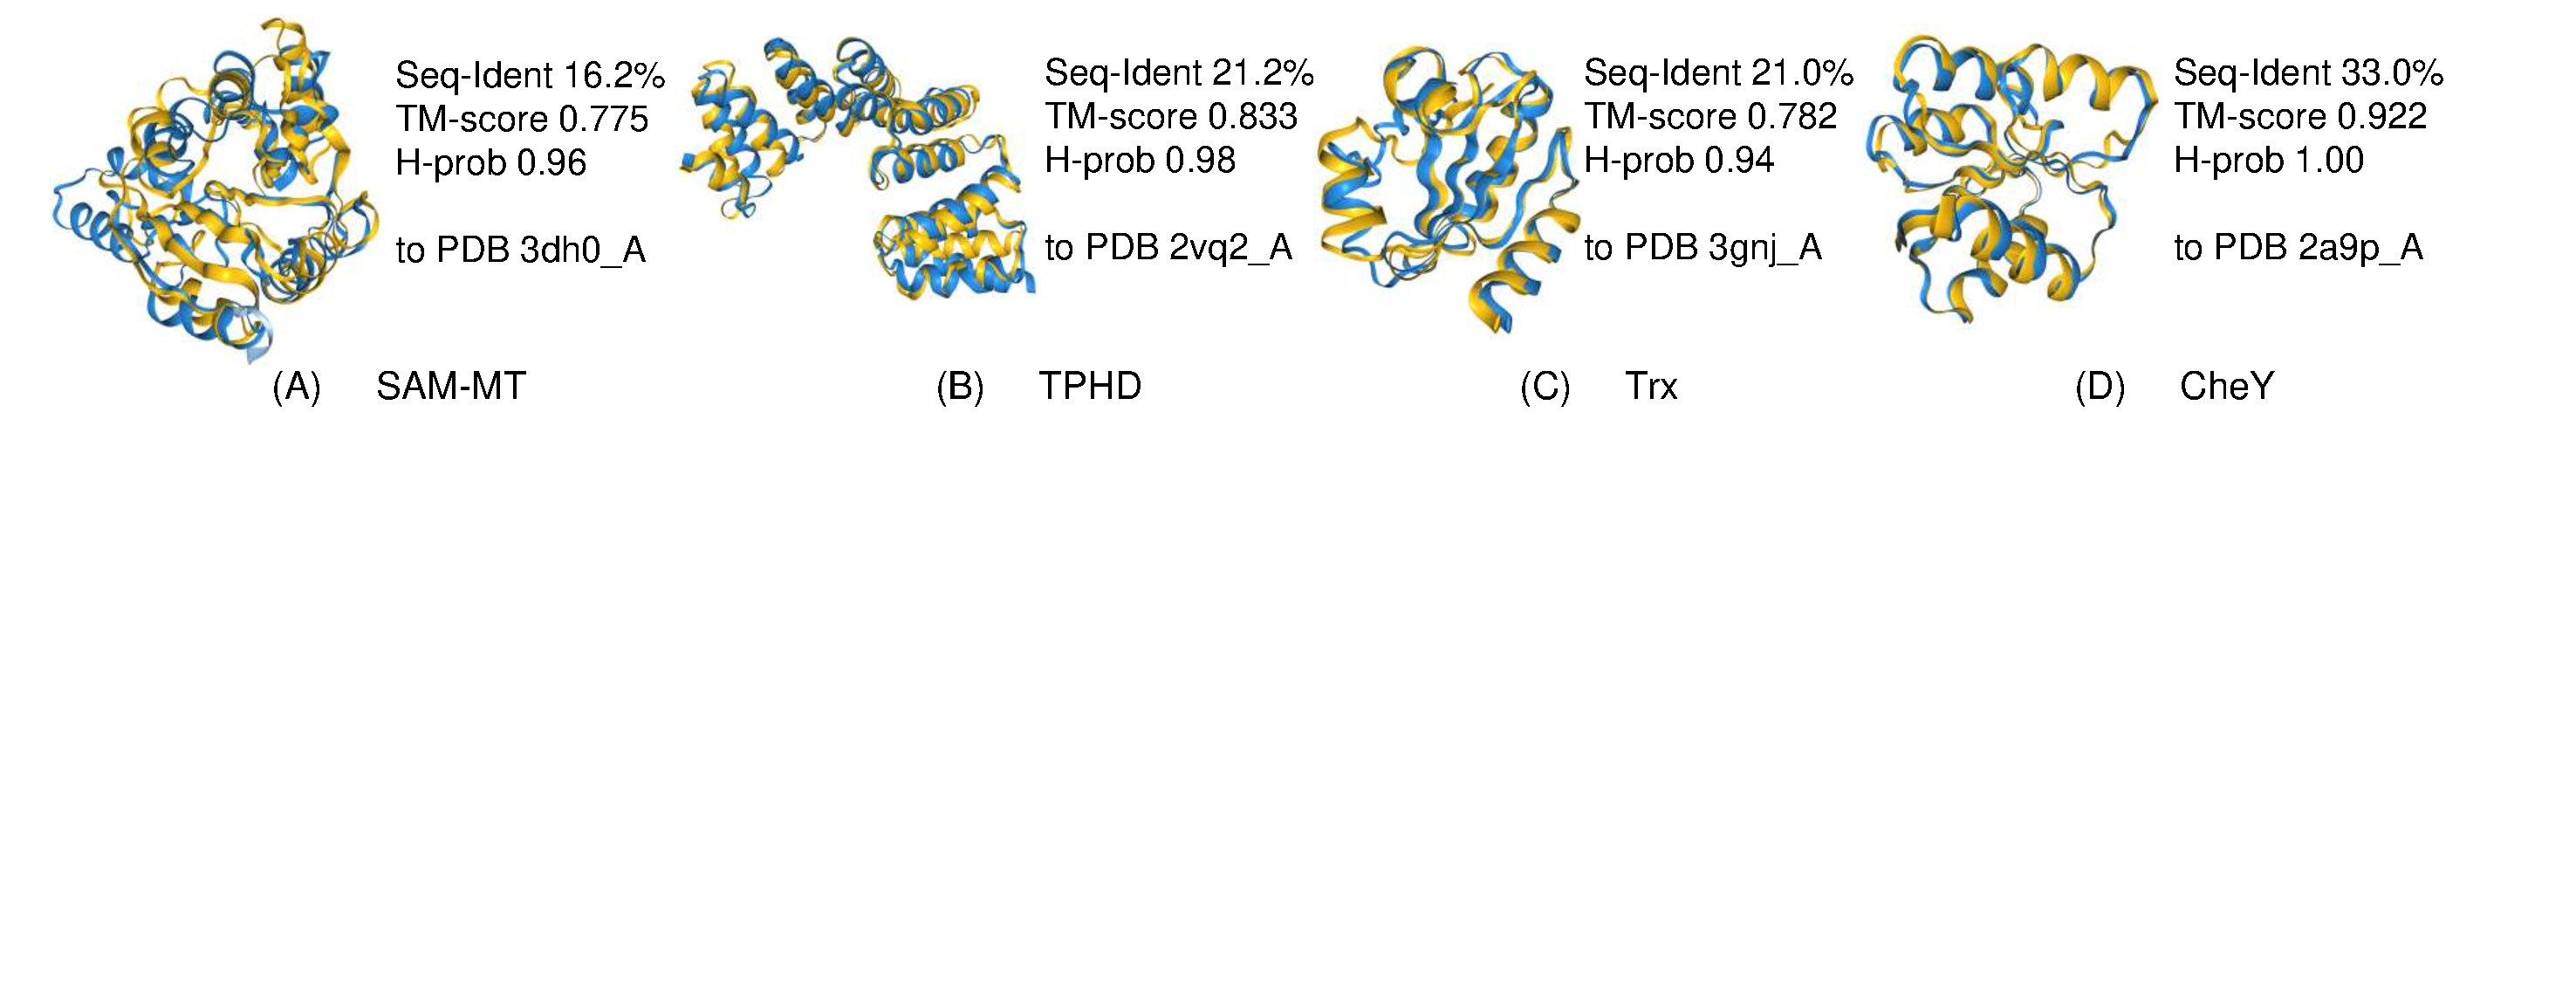
\includegraphics[trim={0 0 90em 0},clip,scale=0.4]{images/protein_visualization.pdf}
		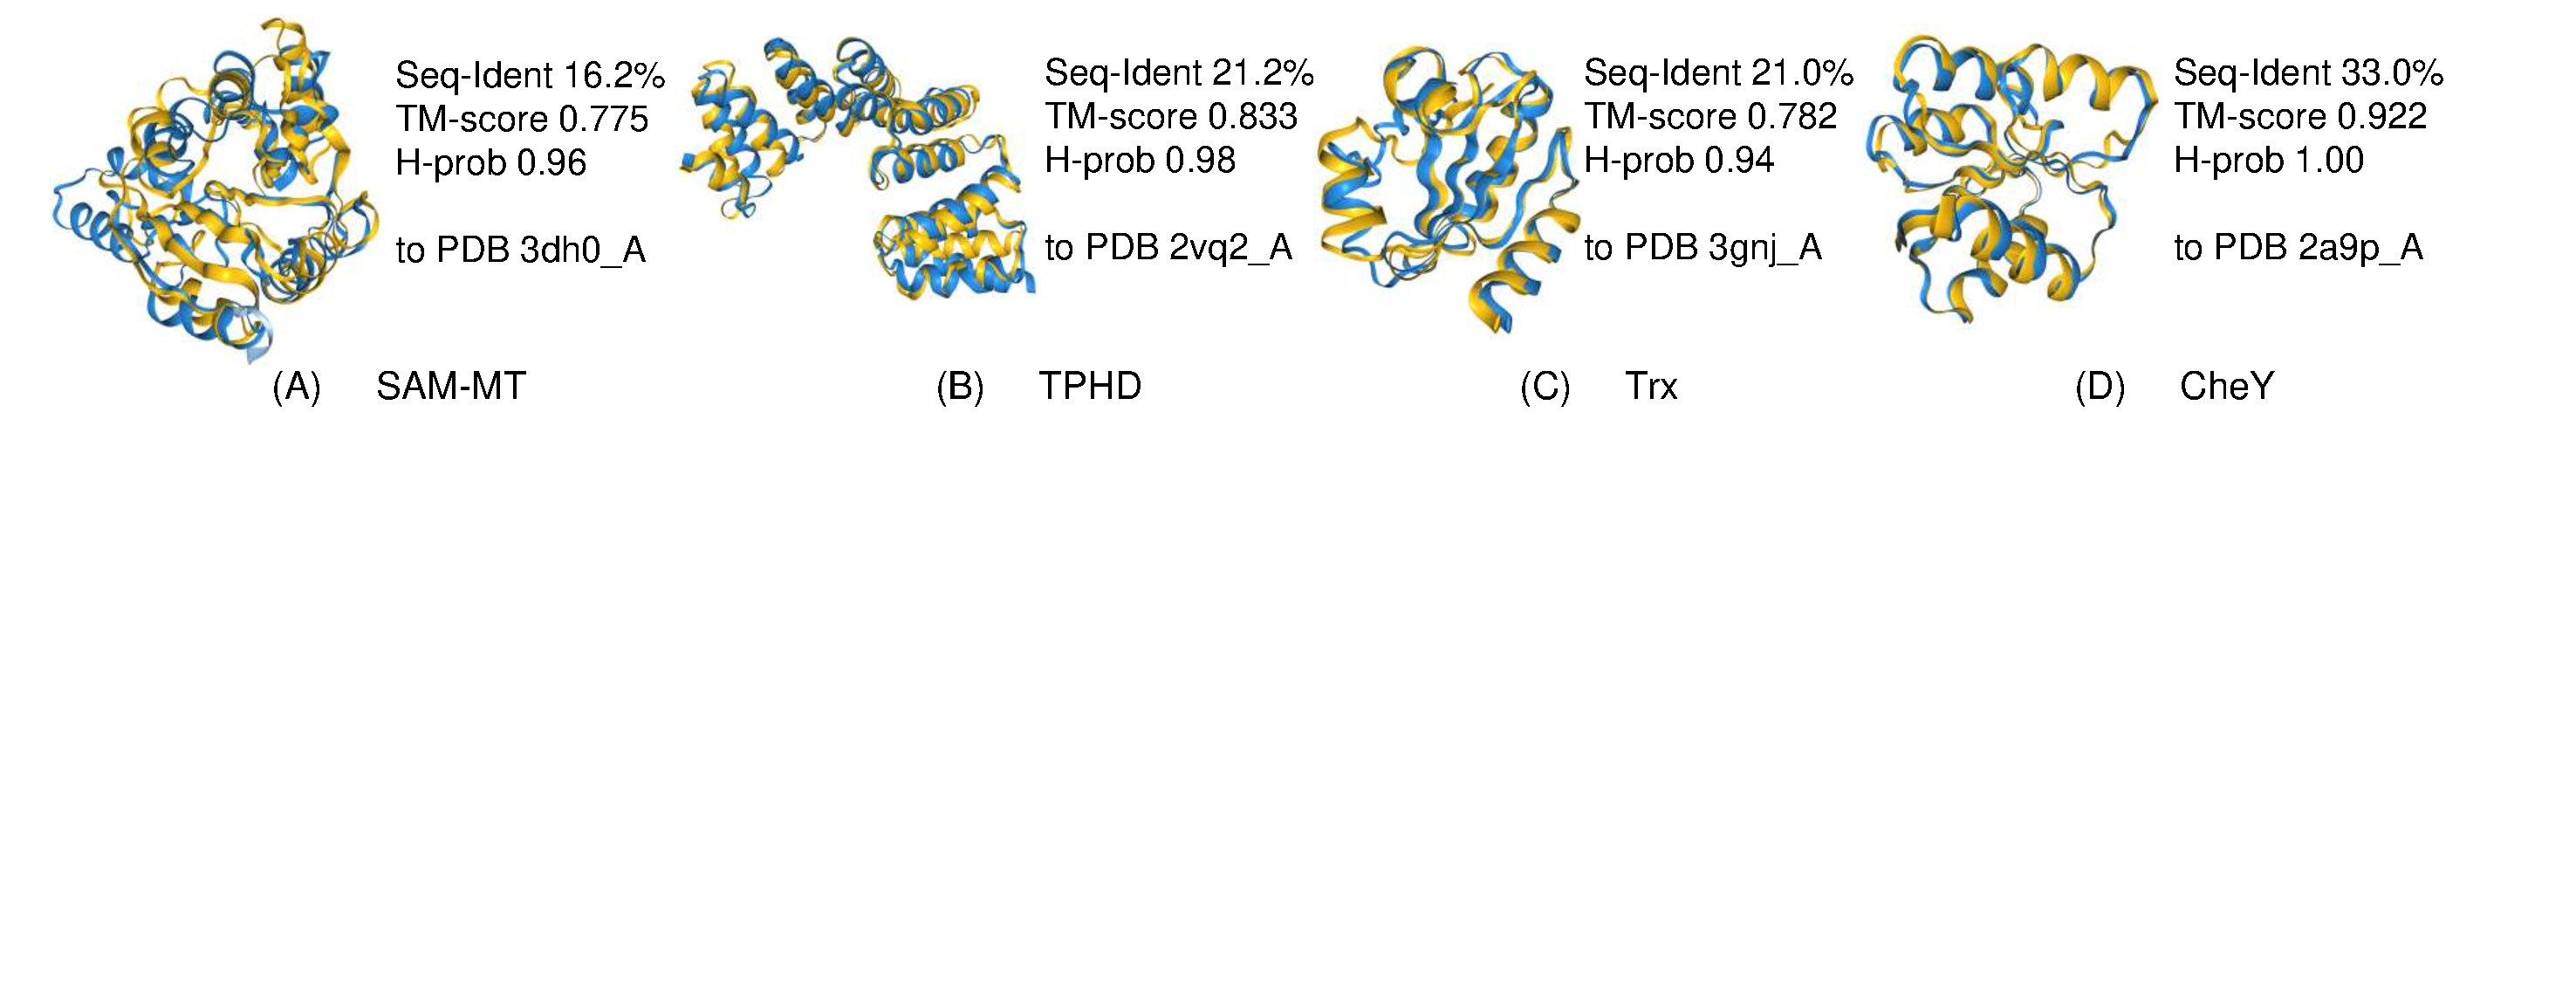
\includegraphics[trim={31.5em 0 57.4em 0},clip,scale=0.4]{images/protein_visualization.pdf}
		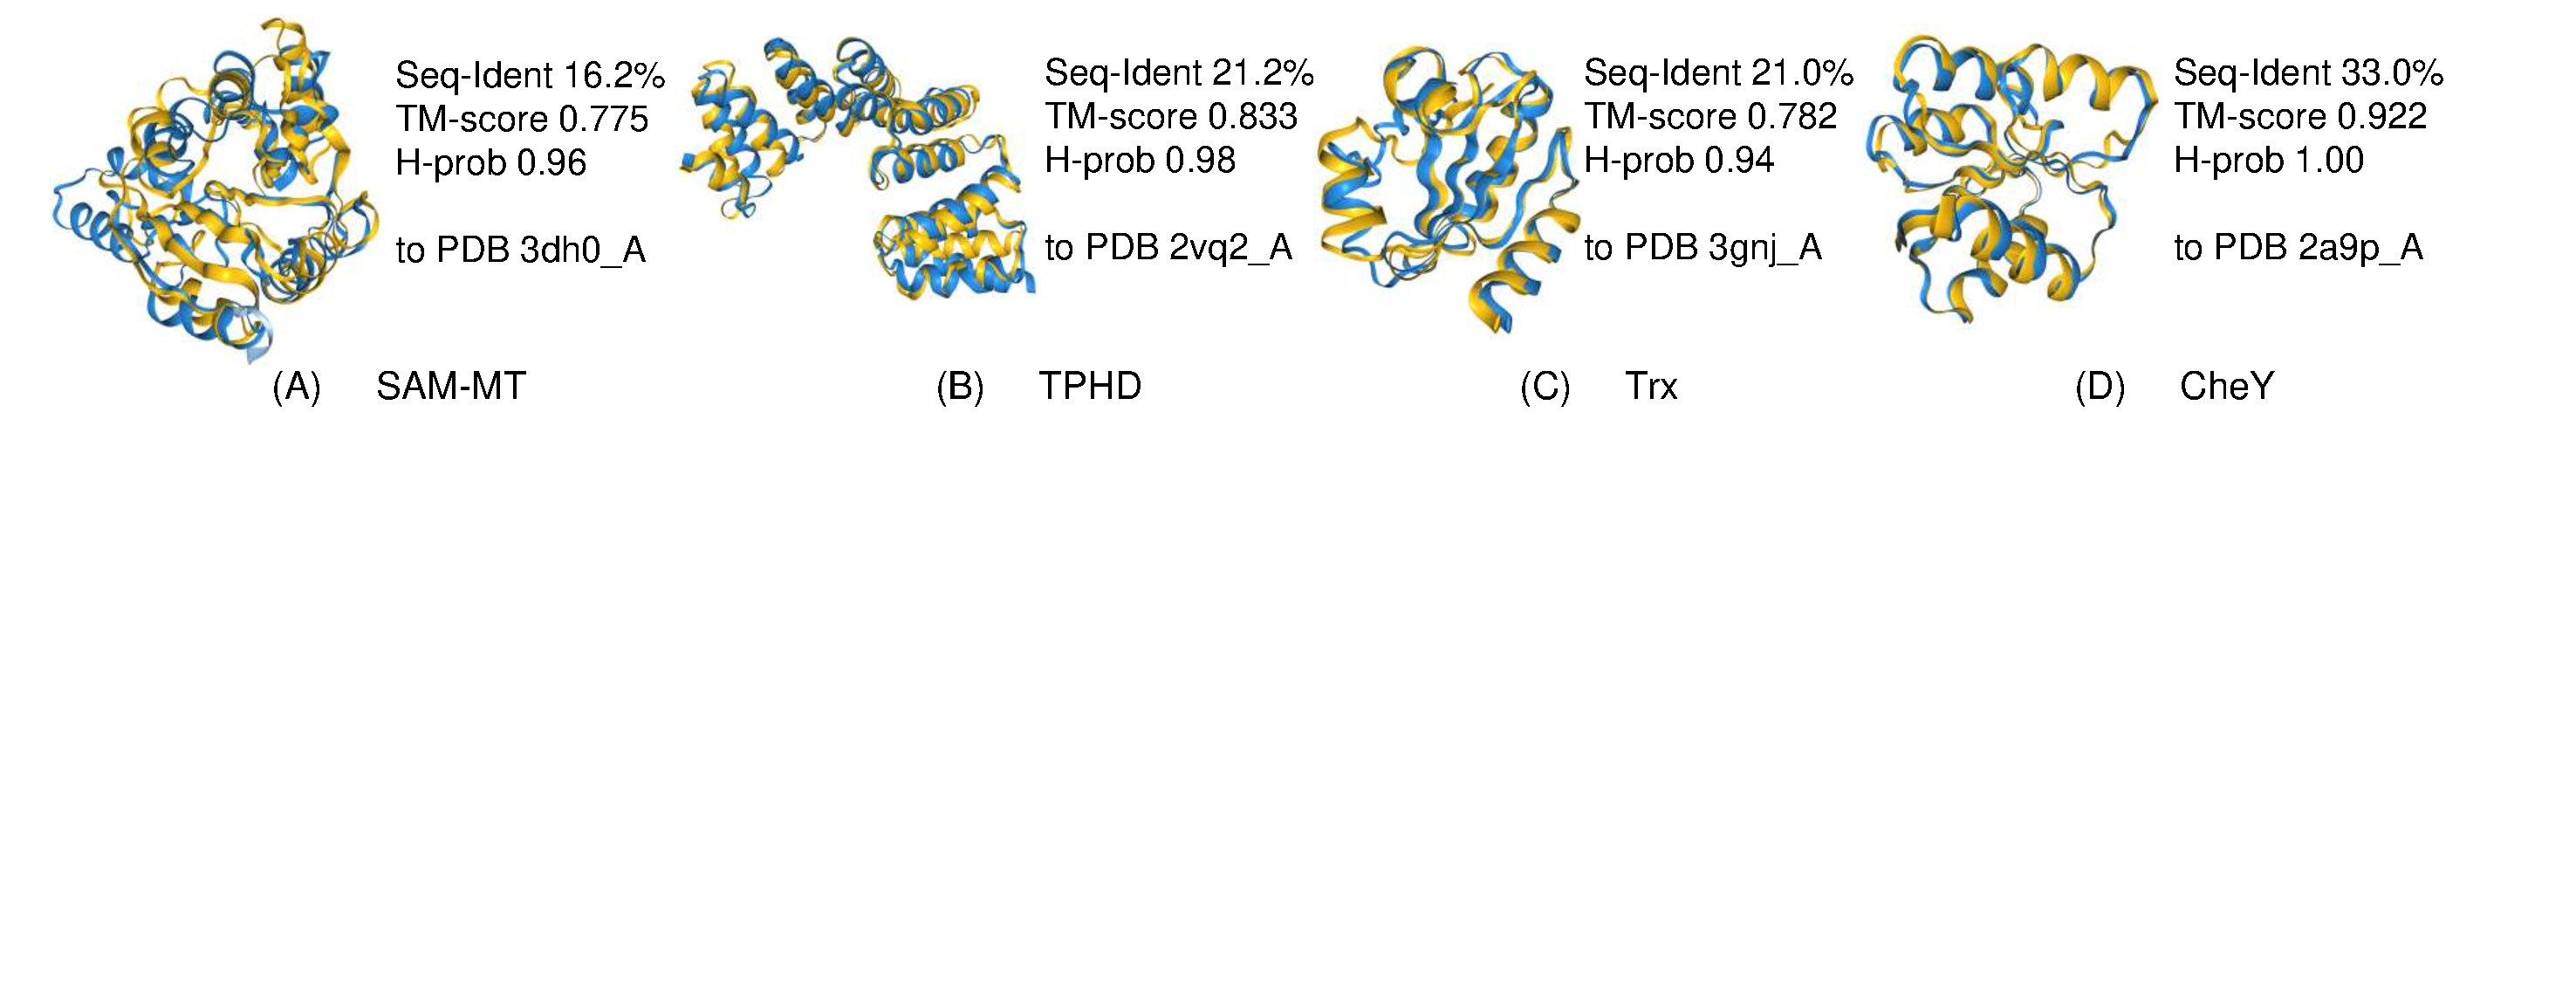
\includegraphics[trim={64em 0 30em 0},clip,scale=0.4]{images/protein_visualization.pdf}
		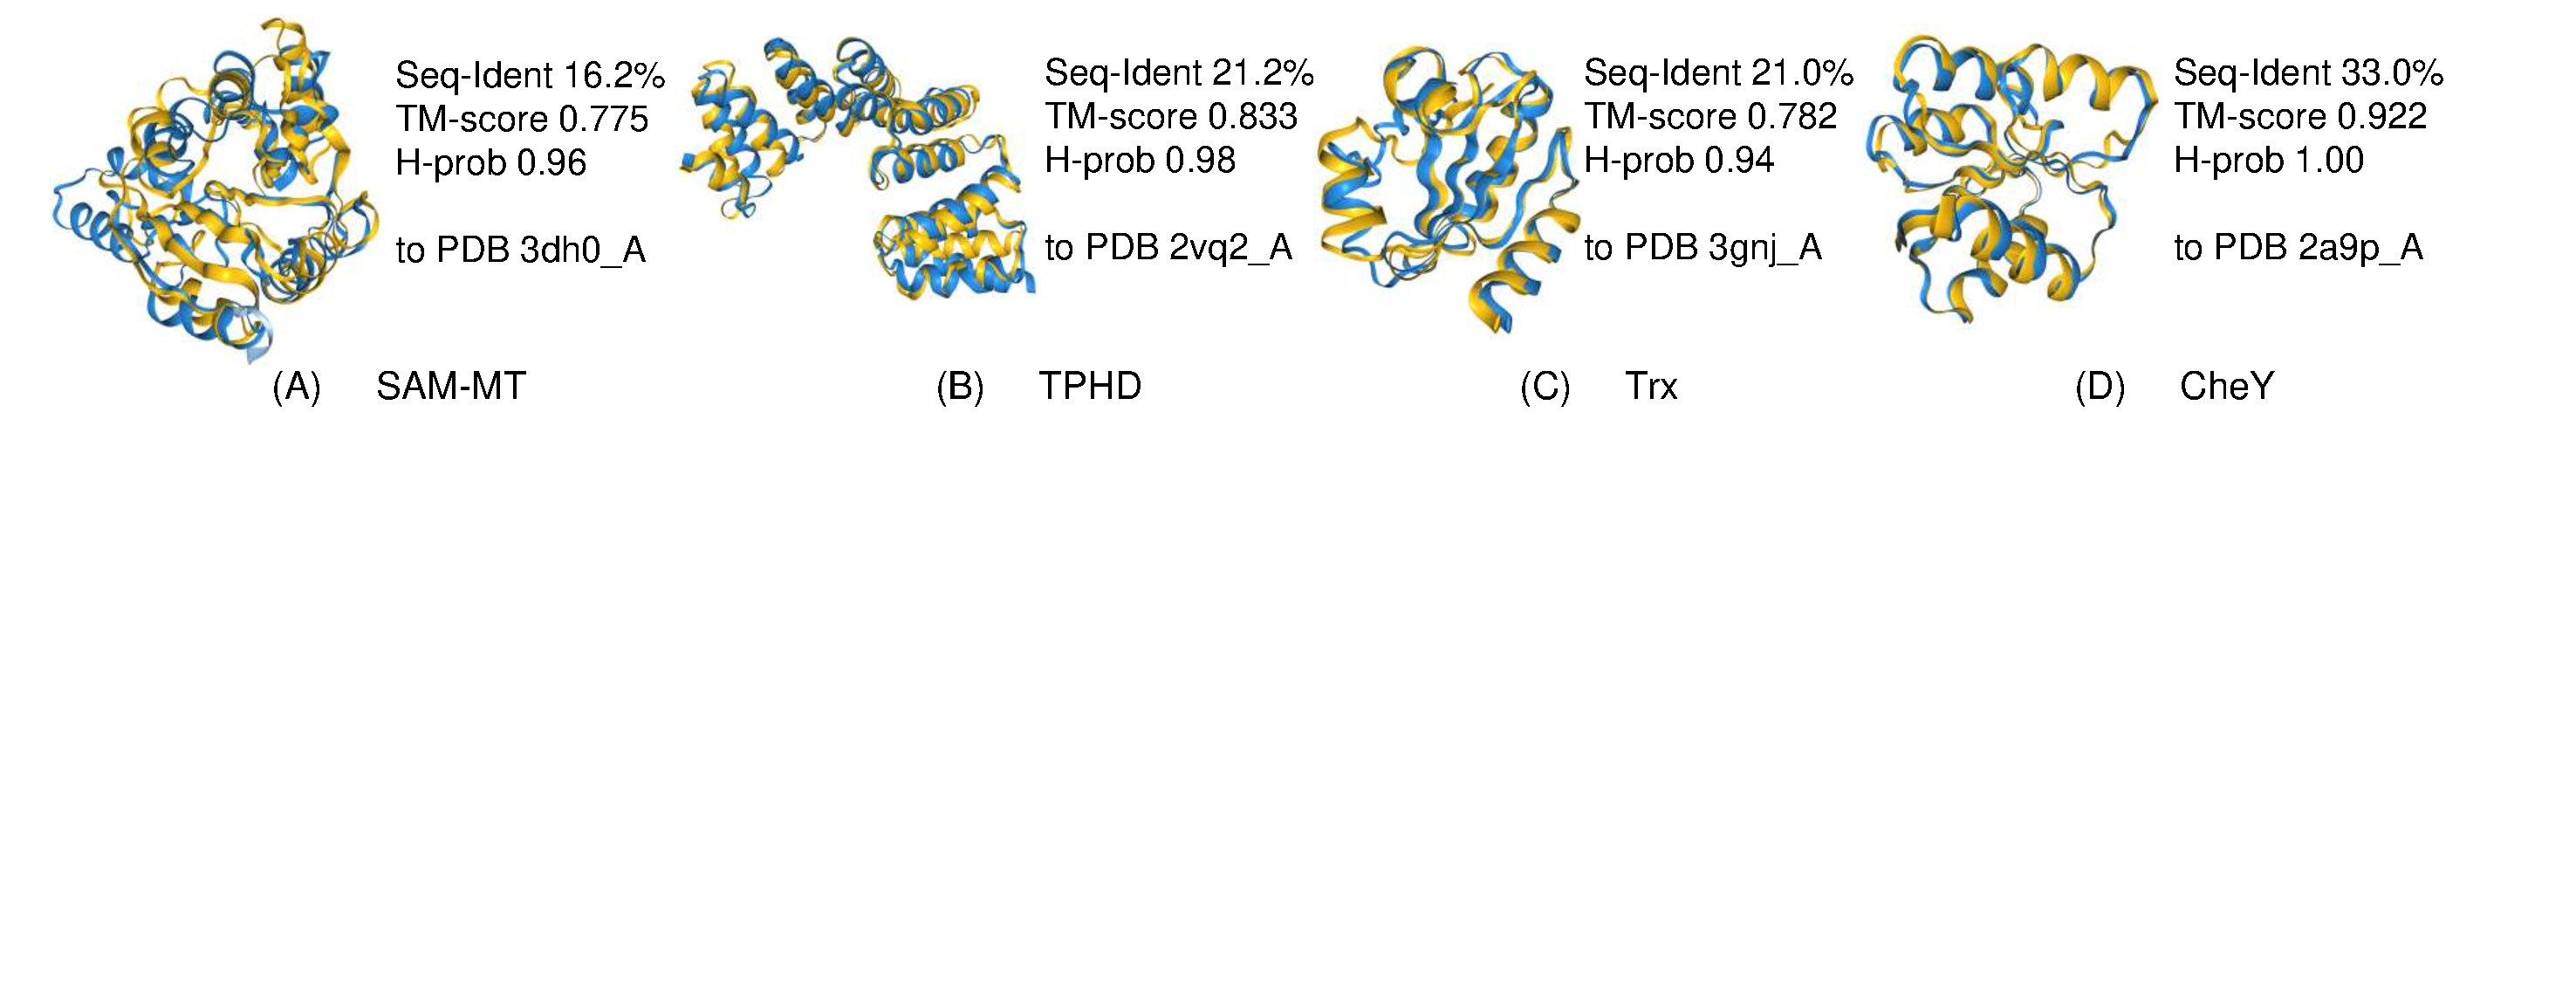
\includegraphics[trim={92em 0 0 0},clip,scale=0.4]{images/protein_visualization.pdf}
	\end{center}
	\vspace{-1em}\credit{Image}{lv2024prollama}
	\begin{itemize}
		\item Blue: generated proteins, yellow: natural proteins
		\item Similar in structure (function), different in sequence
	\end{itemize}
\end{frame}

\begin{frame}{Sequences Generated w/o Instructions - Distributions}
	\begin{center}
		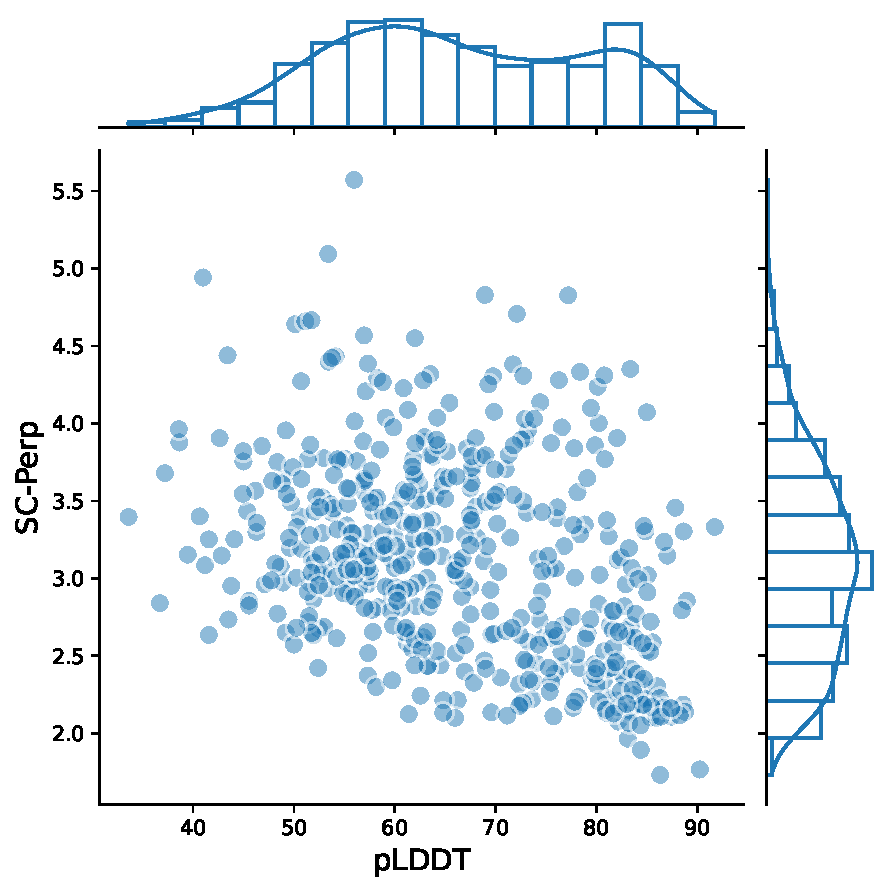
\includegraphics[scale=0.35]{images/plddt_scperp.pdf}
		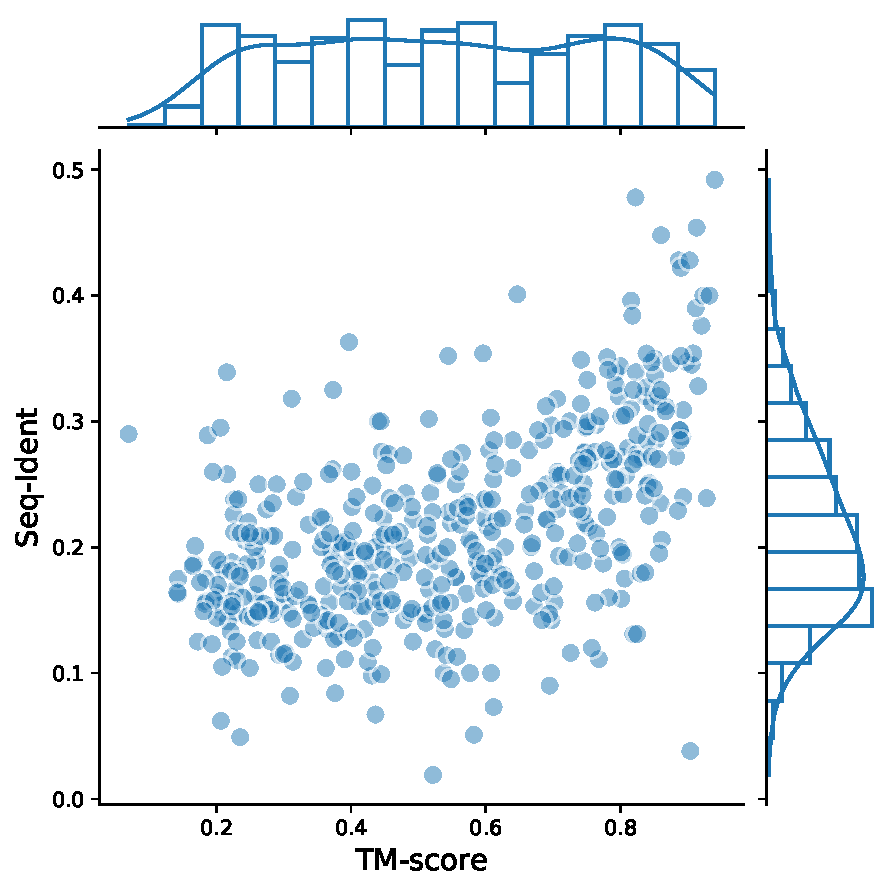
\includegraphics[scale=0.35]{images/tm_sid.pdf}
	\end{center}
	\credit{Image}{lv2024prollama}
	\begin{itemize}
		\item 1 spot = 1 sequence
	\end{itemize}
\end{frame}

\begin{frame}{Natural Language Ability}
	\begin{center}
		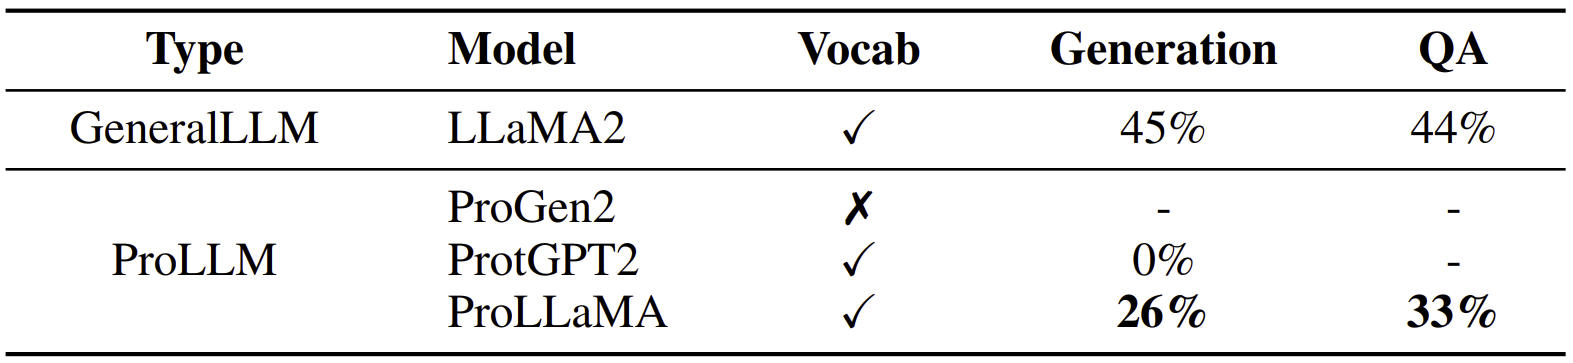
\includegraphics[scale=0.21]{tables/natural_language_ability_comparison.png}
	\end{center}
	\credit{Table}{lv2024prollama}
	\begin{itemize}
		\item Sentence generation on Wikipedia text
	\end{itemize}
\end{frame}

\begin{frame}{Summary}
	\begin{itemize}
		\item Efficient training framework
		\item Can transform any general LLM into a multi-task ProLLM
		\item Versatility
		\begin{itemize}
			\item Unconditional protein generation
			\item Controllable protein generation
			\item Protein property prediction
		\end{itemize}
		\item Exceptional performances
	\end{itemize}
\end{frame}

\section{References}
\begin{frame}[allowframebreaks]
\frametitle{References}
\printbibliography
\end{frame}

\end{document}